\documentclass[12pt]{article}
\usepackage{fullpage,graphicx,psfrag,amsmath,amsfonts,verbatim}
\usepackage[small,bf]{caption}

\input defs.tex

\bibliographystyle{ieeetr}

\title{Bitcoin UTXO Lifespan Prediction}
\author{Robert Konrad \& Stephen Pinto}

\begin{document}
\maketitle

\section{Background \& Motivation}
The Bitcoin crypto currency~\cite{Na08}, born in 2009, still maintains its position as the most widely used and highly valued digital currency in existence. Every day sees thousands of transactions added to the blockchain. The blockchain is a global, agreed-upon ledger of every transaction that has ever occured and is continually extended as a single linked list. Each transaction in the blockchain, say Alice paying Bob 10 BTC, has one or more transaction outputs (TXO) which serve as sums of spendable BTC. These unspent sums are called \emph{Unspent Transaction Outputs} (UTXO). They remain UTXOs until the owner (Bob in our example) redeems them to pay someone else (at which time they are referred to as spent TXOs).

\begin{figure}
\begin{center}
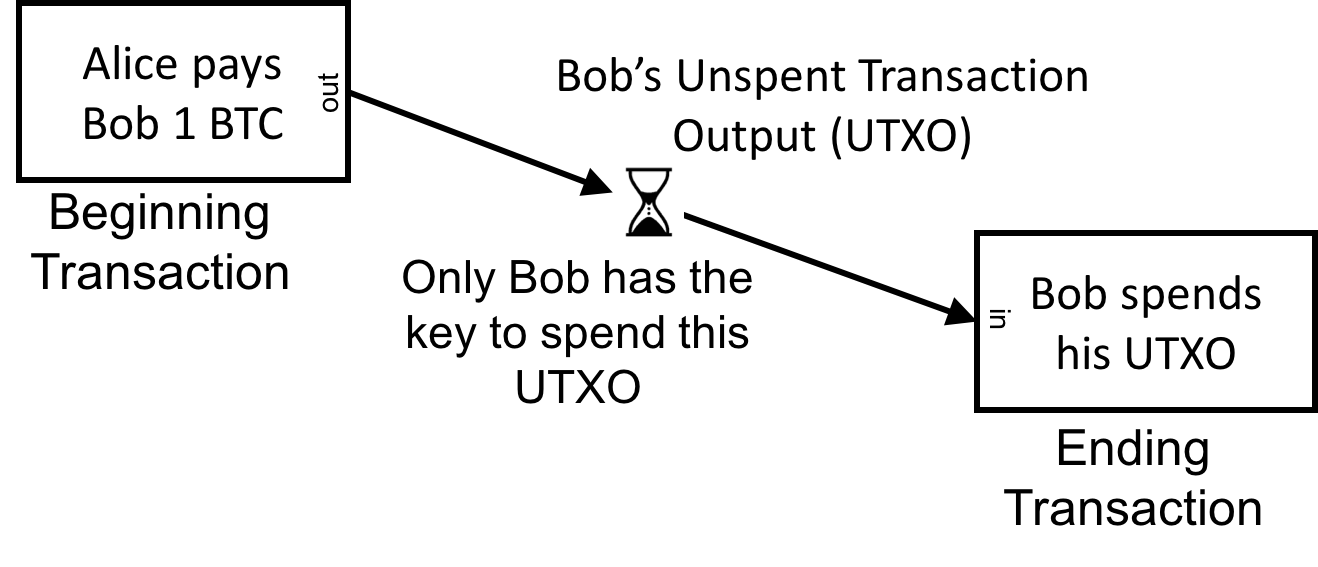
\includegraphics[width=0.7\textwidth]{figures/utxo}
\end{center}
\caption{Illustrated Explanation of a UTXO. An arbitrary amount of time may pass before Bob spends his UTXO.}
\label{utxo}
\end{figure}

This project seeks to predict how long a TXO will remain unspent. More formally, given some information about the beginning transaction which created the UTXO and some information about the Bitcoin market on the day of its creation, this project predicts which of ten broad time scales the UTXO lifespan will fall into. This predictor could inform broader applications such as anomaly/fraud detection, trade volume and volatility prediction, and individual spending habit modelling. The Bitcoin industry is worth billions of dollars and growing rapidly. Possible insights into the previosly mentioned topics would be of use to any number of financial institutions involved in the future of cryptocurrencies. 



\section{Dataset \& Features}
By the nature of Bitcoin's internal structure, every node in the Bitcoin network has a full copy of the blockchain, which has every transaction that has ever occured. We used one of the (many) blockchain exploreres, specifically Blockchain.info, that have a public API exposing data about individual transactions as well as general Bitcoin market statistics. We used HTTP queries in python to gather 13146 training samples and then exported and curated the data in Matlab to gain the features we used during classification.  

\begin{figure}
\begin{center}
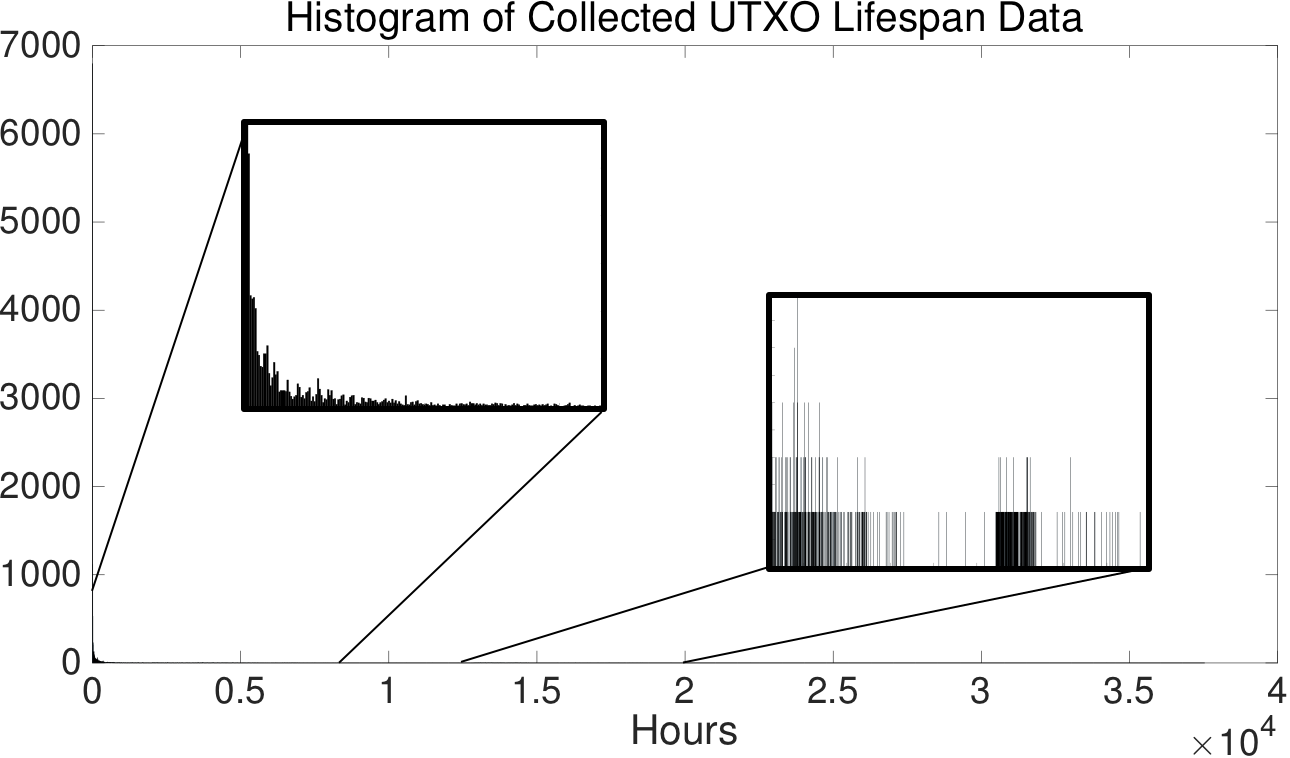
\includegraphics[width=0.9\textwidth]{figures/hist.png}
\end{center}
\caption{The histogram of collected UTXO lifespans with two regions magnified.}
\label{hist}
\end{figure}


\section{Methods}

\begin{figure}
\begin{center}
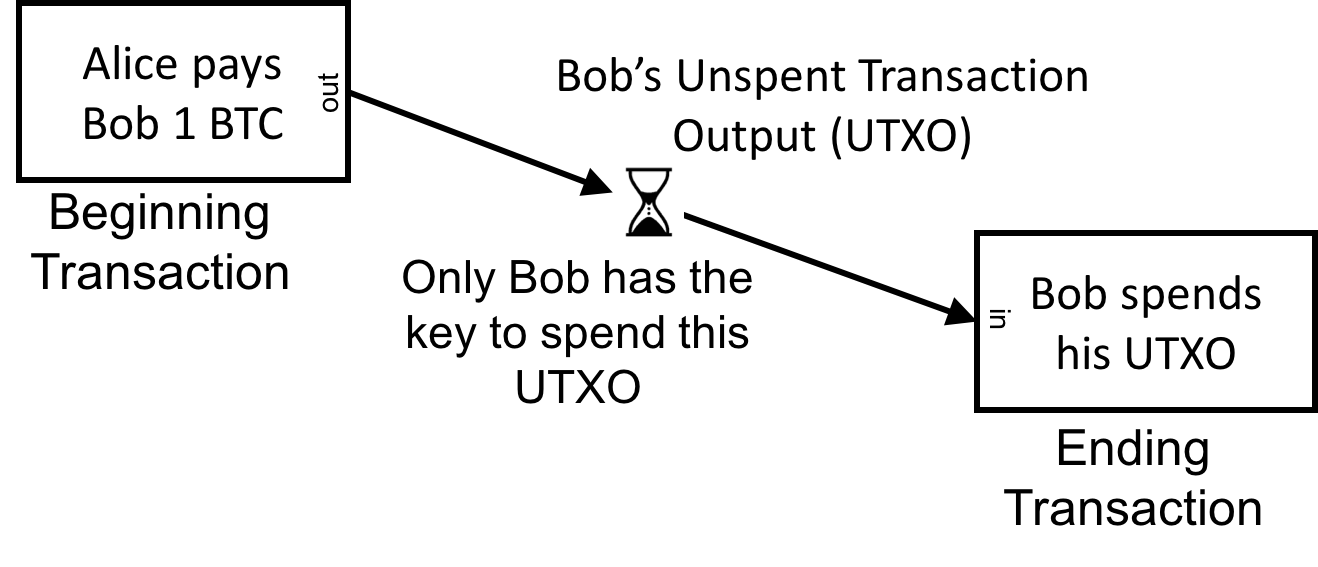
\includegraphics[width=0.9\textwidth]{figures/utxo}
\end{center}
\caption{Illustrated Explanation of a UTXO. An arbitrary amount of time may pass before Bob spends his UTXO.}
\label{utxo}
\end{figure}


\section{Results}

\begin{figure}
\begin{center}
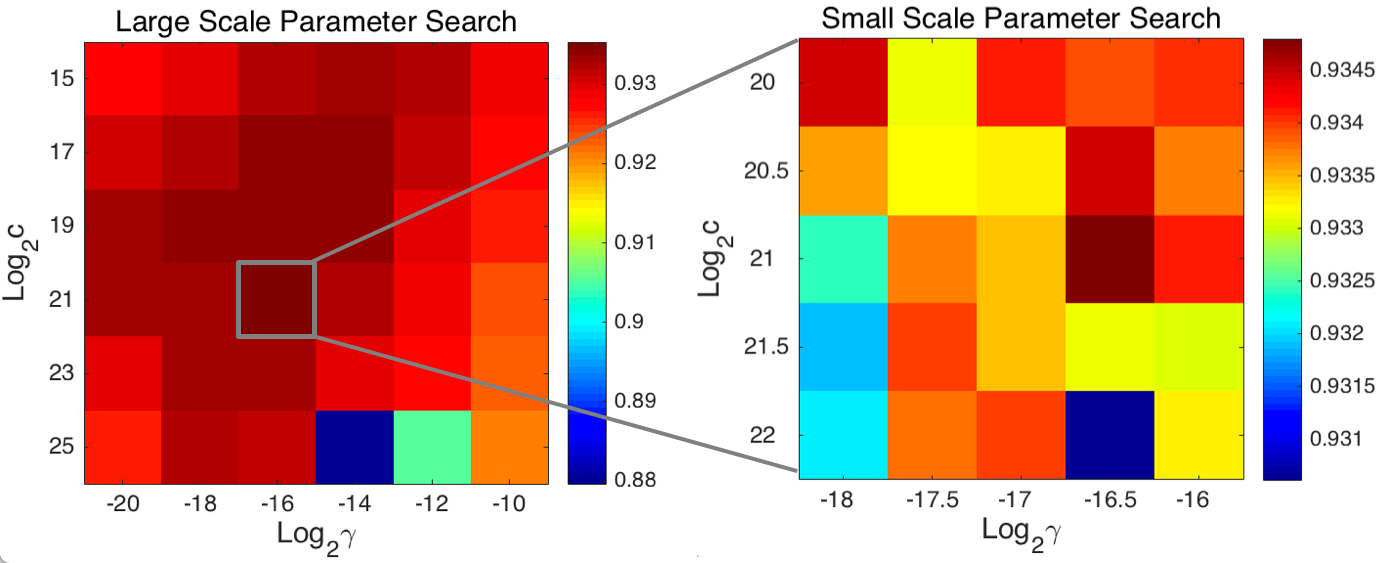
\includegraphics[width=0.9\textwidth]{figures/paramSearch}
\end{center}
\caption{Classifier performance vs $\gamma$ and $C$. One region of the broader heatmap is magnified for higher granularity.}
\label{paramSearch}
\end{figure}

\begin{figure}
\begin{center}
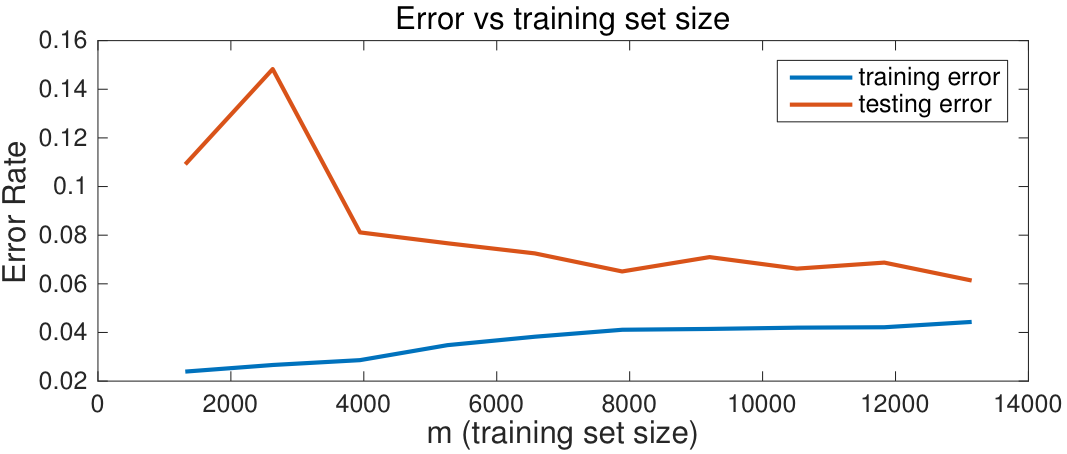
\includegraphics[width=0.9\textwidth]{figures/error}
\end{center}
\caption{Test and training error vs size of data set using 5-fold cross validation.}
\label{error}
\end{figure}

\bibliography{btc-learning}

\end{document}